\chapter{Special Relativity}

\section{Introduction}

The fact that light travels at a finite speed (and not instantaneously fast) has been experimentally known since the 17th century, and by the mid-19th century the numerical value of this speed had been measured with an error of less than 10$\%$. Nevertheless, the question about the precise nature of light had remained unanswered until Maxwell showed in 1861 that electromagnetic waves (oscillatory disturbances in the electric and magnetic fields) propagate in empty space at the speed of $c=3\times10^8$ m/s, precisely the measured value of the speed of light. The prediction that light is a type of electromagnetic wave (just like radio waves and microwaves) was soon verified experimentally, but with this verification new questions arised. First, how can a wave travel in empty space? After all, all the waves known to the physicists of the time were mechanical waves that propagate in materials such as liquids and gases. Second, with respect to what reference frame does light travel with the speed $c$ predicted by 
Maxwell? For if light travels with speed $c$ in some reference frame, then it better have a different speed when measured in some other reference frame that is in motion with respect to the first.\footnote{By reference frame we mean a fixed set of axes $x$, $y$ and $z$, with respect to which the positions of all the bodies in the system are measured as functions of time (it will be useful later to think of the time as another ``axis'' defining the reference frame). A reference frame is also called ``observer,'' ``reference system,'' or simply ``frame'' for short.} To make this point clear, suppose there is an observer who measures the velocity of a particle, which moves along the $x$-axis, to be $u$. Consider a second observer moving (also in the $x$-direction) with speed $v$ relative to the first. What is the speed $u'$ of the particle as measured by this second observer? Any physicist of the 19th century would have answered that
\begin{equation} \label{eq:galilean_vel_rule}
u'=u-v.
\end{equation}
This is called the Galilean velocity addition rule. Although this rule seems to rely on nothing but common sense, it actually relies on an implicit assumption regarding the nature of space and time, an assumption that turns out to be wrong as we will see.

To answer the two questions stated above the physicists of the 19th century proposed the existence of the {\it ether}, an invisible medium that permeates the whole universe. In their view, electromagnetic waves do not really travel in empty space; they are actually supported by the ether, just like sound waves are supported by the air. As for the second question, the speed $c$ predicted by Maxwell is to be measured with respect to the reference frame where the ether is at rest. If this is the case, then we should be able to measure different values of the speed of light in the winter, when the Earth is moving in one direction relative to the ether, and in the summer, when it is moving in the opposite direction. Michelson and Morley attempted to measure this difference in 1887 with completely negative results; the speed of light was measured to be $c$ in every case. Then, in 1905, Einstein came up with a radical solution: the speed of light is $c$ in every inertial reference frame. This clearly contradicts 
the Galilean velocity addition rule (for if $u=c$ then according to Einstein $u'=c$ also, regardless of the value of $v$), as well as many other results of Newtonian physics, as we will see below. This universality of the speed of light implies that the concept of the ether is completely unnecessary; there is no such thing as an absolute reference frame. This also implies that light can indeed travel in empty space; unlike mechanical waves, electromagnetic waves can propagate in vacuum.


\section{The theory of Special Relativity}

Einstein's theory of Special Relativity (SR) is based on the following two basic postulates:
\begin{itemize}
\item [\bf 1.] {\bf The principle of relativity.} The laws of physics apply in the same form in all inertial reference frames.
\item [\bf 2.] {\bf Universality of the speed of light.} The speed of light in vacuum is $c=3\times10^8$ m/s for any observer, regardless of the motion of the light's source relative to the observer.
\end{itemize}

An inertial reference frame is one in which Newton's first law holds: if you are in a frame where particles free of forces move with constant velocity, then the reference frame is inertial,\footnote{You may think that Newton's first law is nothing but a definition, since it states that isolated particles move with uniform velocity in inertial frames. But this is just how inertial frames are defined! However, how do we know that inertial frames actually exist in the first place? The statement that inertial reference frames do exist in the physical world is the true physical content of Newton's first law.} and any other frame moving with constant velocity relative to you will also be inertial. The principle of relativity then states that all these inertial frames are equivalent; there is no absolute reference frame relative to which absolute velocities can be defined.\footnote{Do not confuse the concept of absolute reference frame (like the ether) with that of {\it preferred} reference frame. Many systems of 
course have preferred frames in which its mathematical description is simple. For example, in the case of the solar system, there is a preferred coordinate system in which the Sun sits at the origin with the $z$ axis perpendicular to the plane in which the planets move.} This principle is not really modern; it was originally stated by Galileo in the context of classical mechanics, in which it is a simple consequence of Newton's second law. Indeed, consider a particle of mass $m$ moving with velocity $u(t)$ in some inertial frame (we assume motion in one dimension, say along the $x$ axis). Then Newton's second law states that the force $F$ acting on the particle is related to the velocity by the equation
\begin{equation}
F=ma=m\frac{du}{dt},
\end{equation}
where $a=du/dt$ is the acceleration of the particle. Now consider a second inertial frame moving with velocity $v$ relative to the first. By the Galilean velocity addition rule, eq.\ (\ref{eq:galilean_vel_rule}), the velocity of the particle in this second frame is $u'(t)=u(t)-v$. Notice that $u(t)$ and $u'(t)$ are functions of time (the particle's speed may be changing in time), but $v$ must be a constant for the primed frame to be also inertial. The force and the mass of the particle are (in Newtonian physics) the same in the primed frame, so Newton's second law will read
\begin{equation}
F=ma'=m\frac{du'}{dt}=m\left(\frac{du}{dt}-\frac{dv}{dt}\right)=m\frac{du}{dt},
\end{equation}
where we used that $dv/dt=0$ since $v$ is a constant. We see that Newton's second law has exactly the same form in the second inertial reference frame, consistent with the principle of relativity.

The novelty of Einstein's principle of relativity relies in its application to {\it all} of physics,\footnote{Actually, in the context of Special Relativity we should not include gravity, since it causes some troubles as we will see later. To include gravity one needs the theory of General Relativity.} not just to mechanics. It implies that no experiment of any kind can measure the absolute velocity of a body. In other words, absolute velocity is not an observable quantity, and therefore it is not a true physical concept. The second postulate is even more radical; we already remarked that it contradicts the Galilean velocity addition rule, and in the following we will see other counter-intuitive consequences of the second postulate that will show how the Newtonian notions of space and time have to be modified. But first we need a few definitions. We call an {\it event} something that happens at a single point in space at a single instant in time. An {\it observation} is the act of recording the coordinates 
$x$, $y$, $z$ of the location of an event, and the time $t$ at which the event occurs as indicated by a clock located at the point $(x,y,z)$. Two events are said to be simultaneous if the clocks at the respective locations of the events read the same time (the clocks have to be properly synchronized of course). Notice that making an observation of two simultaneous events is different from {\it seeing} two events occuring at the same instant. For example, consider two light bulbs located at $x_1=3\times10^8$ m and $x_2=6\times10^8$ m; the light bulbs are switched on at $t_1=1$ s and $t_2=0$, respectively. The event of ``first light bulb being switched on'' has the spacetime coordinates $(t_1,x_1)$,\footnote{As noted above, it is useful to think of time as just another coordinate in addition to the spatial coordinates $x$, $y$, $z$. The four dimensions $t$, $x$, $y$, and $z$ define what we call the spacetime. (We will often omit the coordinates $y$ and $z$ when talking about events that occur in one dimension.)
} and the event of ``second light bulb being switched on'' has the spacetime coordinates $(t_2,x_2)$. Since $t_1\neq t_2$ the two events are not simultaneous, although a person sitting at $x=0$ will see the two light bulbs switching on at the same time. There is no contradiction here, of course, since the person is not really observing the original two events (``light bulbs switching on''), but the different events of ``light beams reaching $x=0$'' which have coordinates $(t=2~{\rm s},x=0)$.

\subsection{The relativity of simultaneity}

Consider a train car traveling at constant speed along a straight, frictionless track (fig.\ \ref{fig:lec2_1}). At the middle point of the car there is a light bulb. The bulb is switched on at some instant, emitting two light rays in the front and back directions. Clearly, an observer on the train will find that the rays reach the front and back ends of the car at the same time, since the light bulb is equidistant from the two ends, and the rays both travel with the same speed $c$. Let us define as event $A$ when the ray reaches the front end, and as event $B$ when the other ray reaches the back end. Then, according to the observer on the train, events $A$ and $B$ are simultaneous. Now consider these same two events from the point of view of an observer on the ground. The light rays both travel with the same speed $c$ (from postulate 2), but since the train car is moving, the ray moving in the front direction will have to travel a distance larger than half of the length of the car, whereas the opposite is 
true for the ray moving in the back direction. The observer on the ground would then find that event $B$ happens before event $A$, thereby concluding that the two events are not simultaneous.
\begin{figure}[ht]
\begin{center}
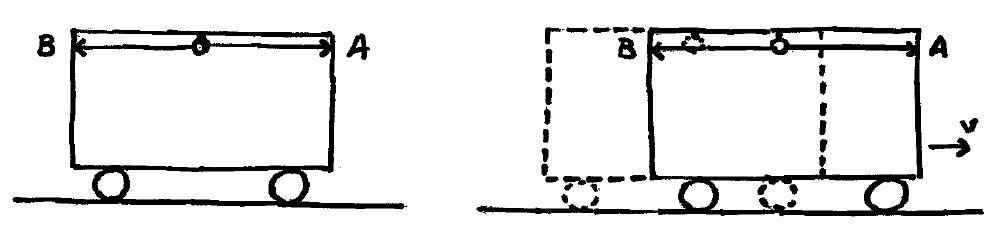
\includegraphics[scale=0.5]{Draw/lec2_1.png}
\end{center}
\caption{Relativity of simultaneity}
\label{fig:lec2_1}
\end{figure}

This example illustrates the concept of the relativity of simultaneity: two events that are simultaneous in one inertial reference frame are not, in general, simultaneous in another. It is a direct consequence of the postulate of the universality of the speed of light. Notice that, for this effect to be important, the train in the above example would have to be moving extremely fast, for otherwise the difference in the distances the two light rays must travel, as seen by the ground observer, would be extremely small. This is due to the fact that the speed of light is so much larger than any of the speeds involved in everyday life, which is why we do not easily notice this and other relativistic effects.

\subsection{Time dilation}

Consider again the train car of the previous example (which we will call system $S'$), but now suppose the light bulb sends a ray directed straight down to the floor of the car. If the height of the car is $h$, then the time it takes the light ray to reach the floor is
\begin{equation}
\Delta t'=\frac{h}{c}.
\end{equation}
\begin{figure}[ht]
\begin{center}
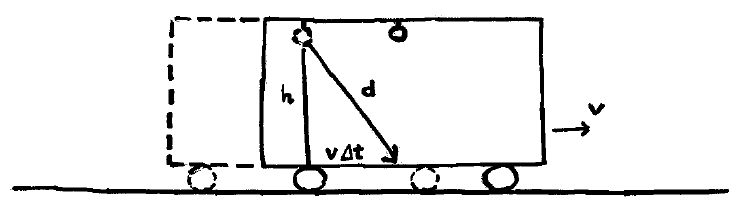
\includegraphics[scale=0.6]{Draw/lec2_2.png}
\end{center}
\caption{Time dilation}
\label{fig:lec2_2}
\end{figure}

\noindent
On the other hand, for the observer on the ground (system $S$) the light ray does not travel straight down, since the car has moved a distance $v\Delta t$ by the time the ray reaches the floor of the car. Here $\Delta t$ is the time interval as measured by the ground observer, $v$ is the speed of the train, and we have again used postulate 2 in assuming that the light ray travels with speed $c$. From fig.\ \ref{fig:lec2_2} we can see that the distance the light ray travels is given by
\begin{equation}
d=\sqrt{h^2+(v\Delta t)^2},
\end{equation}
so that the time it takes the ray to make the trip is
\begin{equation}
\Delta t=\frac{d}{c}=\frac{\sqrt{h^2+(v\Delta t)^2}}{c}.
\end{equation}
We can solve this equation for $\Delta t$, finding that
\begin{equation}
\Delta t=\frac{h}{c}\frac{1}{\sqrt{1-v^2/c^2}}.
\end{equation}
Also, since $\Delta t'=h/c$, we can write this as
\begin{equation} \label{eq:time_dilation}
\Delta t=\frac{\Delta t'}{\sqrt{1-v^2/c^2}}.
\end{equation}
Notice that $\Delta t>\Delta t'$, meaning that for the observer on the ground the time interval between the two events (``light ray being emitted,'' and ``light ray reaches the floor'') is larger than the time interval measured by the observer on the train. This is the phenomenon of time dilation, which is often summarized by the statement ``moving clocks run slow.''

\subsection{Lorentz contraction}

Once again we consider the train car traveling with speed $v$ relative to the ground. Imagine now that there is a flashlight located at the back end of the car, and a mirror at the front end, so that a light ray sent by the flashlight will make a round trip along the car (fig.\ \ref{fig:lec2_3}). For an observer on the train, the time it takes the ray to make the trip is
\begin{equation}
\Delta t'=2\frac{L_0}{c},
\end{equation}
where $L_0$ is the {\it rest length} of the train car, i.e.\ the length of the car as measured in the reference frame where it is at rest. We want to compute now this time interval as measured by an observer on the ground. Let $\Delta t_1$ be time for the light ray to reach the mirror, and $\Delta t_2$ the time to return to the back end. If the car has a length $L$ in the ground system, then the ray travels a distance $d_1=L+v\Delta t_1$ from the back to the front, since by the time it reaches the front end the train has moved a distance $v\Delta t_1$. Similarly, the light ray travels a distance $d_2=L-v\Delta t_2$ from the front to the back, since by the time the ray arrives to the back end the train has moved a distance $v\Delta t_2$ (convince yourself that this distance has to be subtracted, so that $d_2$ is shorter than $L$). The time intervals in the ground frame are therefore
\begin{equation}
\Delta t_1=\frac{L+v\Delta t_1}{c},~~~~~~~~\Delta t_2=\frac{L-v\Delta t_2}{c}.
\end{equation}
Solving for $\Delta t_1$ and $\Delta t_2$ from these equations we find
\begin{equation}
\Delta t_1=\frac{L}{c-v},~~~~~~~~\Delta t_2=\frac{L}{c+v}.
\end{equation}
\begin{figure}[ht]
\begin{center}
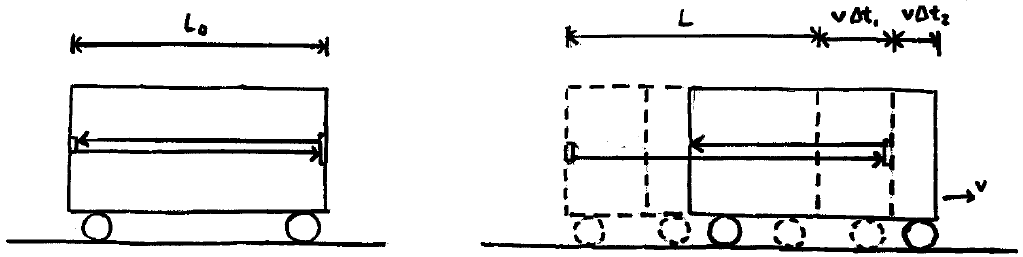
\includegraphics[scale=0.6]{Draw/lec2_3.png}
\end{center}
\caption{Lorentz contraction}
\label{fig:lec2_3}
\end{figure}

\noindent
The total time for the round trip is then
\begin{equation}
\Delta t=\Delta t_1+\Delta t_2=2\frac{L}{c}\frac{1}{(1-v^2/c^2)}.
\end{equation}
But we also know, from eq.\ (\ref{eq:time_dilation}), that the time intervals are related by $\Delta t'=\sqrt{1-v^2/c^2}\Delta t$. Applying this to the times we just found, we get
\begin{equation}
 2\frac{L_0}{c}=2\frac{L}{c}\frac{\sqrt{1-v^2/c^2}}{(1-v^2/c^2)},
\end{equation}
or
\begin{equation}
L=\sqrt{1-v^2/c^2}L_0.
\end{equation}
Notice that $L$, the length of the car observed from the ground, is shorter than $L_0$, the length of the car as measured in the frame where the car is at rest. This is the phenomenon of Lorentz contraction, which can be summarized with the sentence ``moving objects are shortened.'' It is important to note that the contraction only occurs along the direction of motion; the dimensions perpendicular to the velocity are unchanged.

\section{The Lorentz transformations}

Consider an event with coordinates $(t,x,y,z)$ in some inertial reference system $S$. We would like to find the coordinates $(t',x',y',z')$ of this same event in some other inertial system $S'$. Suppose the system $S'$ is moving with constant speed $v$ relative to the system $S$, along the positive $x$-direction. We assume that the $x$ and $x'$ axes are parallel, and that the origins $O$ and $O'$ of the two systems coincide at $t=t'=0$; see fig.\ \ref{fig:lec2_4}. Let us go back to Newtonian physics for a moment, where the time is absolute and runs at the same rate in all inertial frames. This means that $t'=t$ for the event we are considering. It is clear then, from fig.\ \ref{fig:lec2_4}, that the coordinates $(t',x',y',z')$ of the event are related to the coordinates $(t,x,y,z)$ by the equations
\begin{equation}
\begin{split}
x'&=x-vt,\\
y'&=y,\\
z'&=z,\\
t'&=t.\\
\end{split}
\end{equation}
These are called the Galilean transformations.\footnote{Notice that the Galilean velocity addition rule, eq.\ (\ref{eq:galilean_vel_rule}), follows from taking the time derivative of the first equation.} Although they seem to be quite obvious at first sight, we should not forget that we derived them from the assumption that time runs at the same rate in all inertial systems. But we now know that this is not true; we have seen how Einstein's second postulate forces us to abandon the notion of absolute time, implying that the Galilean transformations have to be modified to account for the universality of the speed of light. The correct equations read
\begin{equation} \label{eq:lorentz_transf}
\begin{split}
x'&=\gamma\left(x-vt\right),\\
y'&=y,\\
z'&=z,\\
t'&=\gamma\left(t-\frac{v}{c^2}x\right).\\
\end{split}
\end{equation}
The parameter $\gamma$ is defined as
\begin{equation}
\gamma\equiv\frac{1}{\sqrt{1-v^2/c^2}}.
\end{equation}
These are known as the Lorentz transformations. Notice that whenever $v\ll c$ (so that $\gamma\approx1$) these reduce to the Galilean transformations. This is why we can safely apply Newtonian physics as long as we deal with speeds much smaller than the speed of light.
\begin{figure}[ht]
\begin{center}
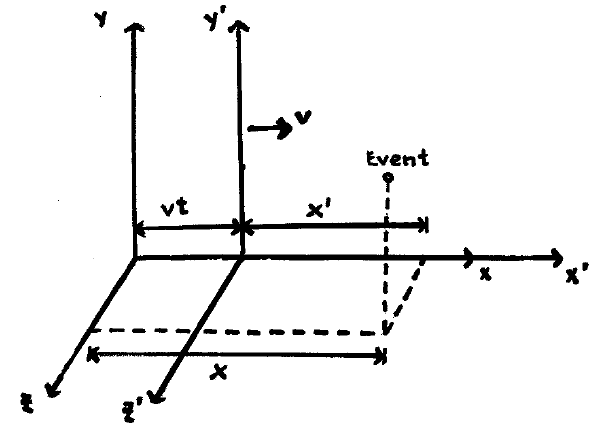
\includegraphics[scale=0.5]{Draw/lec2_4.png}
\end{center}
\caption{Galilean transformations}
\label{fig:lec2_4}
\end{figure}

Next consider two events separated in space by the distances $(\Delta x,\Delta y,\Delta z)$ and in time by the interval $\Delta t$, as measured in the system $S$. For definiteness, we can think of the two events as ``a particle located at the spacetime point $(t,x,y,z)$'' and ``the same particle located at the spacetime point $(t+\Delta t,x+\Delta x,y+\Delta y,z+\Delta z)$,'' so that we keep track of the particle's motion by means of two events. Now we can apply the Lorentz transformations to these two events and find their coordinates in the system $S'$. One can then show that, by subtracting the equations for the two events, the intervals $\Delta t'$, $\Delta x'$, $\Delta y'$, and $\Delta z'$ measured in the frame $S'$ are given by
\begin{equation} \label{eq:lorentz_intervals}
\begin{split}
\Delta x'&=\gamma\left(\Delta x-v\Delta t\right),\\
\Delta y'&=\Delta y,\\
\Delta z'&=\Delta z,\\
\Delta t'&=\gamma\left(\Delta t-\frac{v}{c^2}\Delta x\right).\\
\end{split}
\end{equation}
Suppose the particle is moving in the $x$-direction, so that $\Delta y=\Delta y'=0$ and $\Delta z=\Delta z'=0$. We can compute the ratio $\Delta x'/\Delta  t'$ from these equations as follows:
\begin{equation}
\frac{\Delta x'}{\Delta t'}=\frac{\gamma\left(\Delta x-v\Delta t\right)}{\gamma\left(\Delta t-\frac{v}{c^2}\Delta x\right)}=\frac{\frac{\Delta x}{\Delta t}-v}{1-\frac{v}{c^2}\frac{\Delta x}{\Delta t}}.
\end{equation}
But $\Delta x/\Delta t\equiv u$ is equal to the velocity of the particle in the system $S$, whereas $\Delta x'/\Delta t'\equiv u'$ is its velocity in the system $S'$. The above equation then tells us how to relate $u$ and $u'$:
\begin{equation} \label{eq:einstein_vel_rule}
u'=\frac{u-v}{1-\frac{vu}{c^2}}.
\end{equation}
This is known as Einstein's velocity addition rule, which is the analog of the Galilean rule in SR. Note that if $u\ll c$ and $v\ll c$ Einstein's rule reduces to the Galilean rule, as it should. To check that this formula is consistent with the universality of the speed of light, suppose the particle is a photon, so that $u=c$ in the system $S$. Then its speed in the system $S'$ is
\begin{equation}
u'=\frac{c-v}{1-\frac{v}{c}}=c,
\end{equation}
so that indeed the photon has a speed $c$ in all reference frames.

\par\vspace{\baselineskip}

{\bf Exercise.} Derive the formulas for time dilation and Lorentz contraction starting from the Lorentz transformations.

\section{The spacetime interval}

Given two events separated in spacetime by $(\Delta t,\Delta x,\Delta y,\Delta z)$, as measured in some inertial reference system $S$, we define the {\it spacetime interval} between the events as
\begin{equation}
\Delta s^2=-c^2\Delta t^2+\Delta x^2+\Delta y^2+\Delta z^2.
\end{equation}
We would like to know how does this spacetime interval change when we consider the same two events in a reference frame $S'$ that moves with velocity $v$ relative to $S$ in the $x$-direction (with the respective axes parallel, just as in the previous section). To answer this we simply have to compute the interval $\Delta s'^2$ using the Lorentz transformations of eq.\ (\ref{eq:lorentz_intervals}):
\begin{equation}
\begin{split}
\Delta s'^2&=-c^2\Delta t'^2+\Delta x'^2+\Delta y'^2+\Delta z'^2\\
&=-c^2\left[\gamma\left(\Delta t-\frac{v}{c^2}\Delta x\right)\right]^2+\left[\gamma\left(\Delta x-v\Delta t\right)\right]^2+\Delta y^2+\Delta z^2\\
&=\Delta t^2\left[-\gamma^2c^2+\gamma^2v^2\right]+\Delta x^2\left[-\gamma^2\frac{v^2}{c^2}+\gamma^2\right]+\Delta x\Delta t\left[2c^2\gamma\frac{v}{c^2}-2\gamma v\right]+\Delta y^2+\Delta z^2\\
&=-c^2\Delta t^2+\Delta x^2+\Delta y^2+\Delta z^2.
\end{split}
\end{equation}
Thus we have obtained the very important result
\begin{equation}
\Delta s'^2=\Delta s^2,
\end{equation}
which states that the spacetime interval between two events has the same value in all inertial reference frames. We say that $\Delta s^2$ is {\it invariant} under Lorentz transformations. In the modern point of view, the invariance of the interval is often taken as the starting point of SR.\footnote{We showed that $\Delta s^2$ is invariant by using the Lorentz transformations, but it turns out that one can also do the opposite, that is, to derive the Lorentz transformations starting from the invariance of the interval.} The reason for this is that, as we will see later, the interval allows us to understand spacetime in a geometrical way, which will be useful when we move on to study General Relativity. To see how to use the interval in practice, we will now rederive the formulas of time dilation and Lorentz contraction by exploiting the invariance of $\Delta s^2$.

\subsection{Time dilation again}

Consider a train (system $S'$) moving with speed $v$ relative to the platform (system $S$), as shown in fig.\ \ref{fig:lec2_5}. There is a clock traveling on the train, and we want to find the time elapsed between two successive ticks as measured in $S$ and in $S'$. We do this by computing the spacetime interval between the two events (first tick and second tick) in the respective reference systems.
\begin{figure}[ht]
\begin{center}
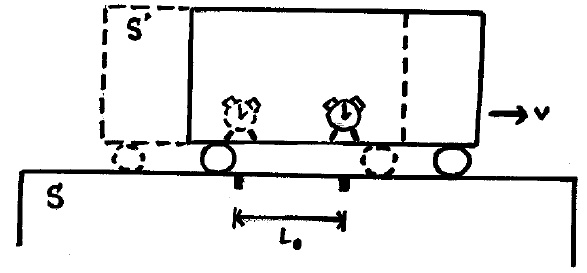
\includegraphics[scale=0.6]{Draw/lec2_5.png}
\end{center}
\caption{The spacetime interval}
\label{fig:lec2_5}
\end{figure}

For an observer on the train $\Delta x'=0$, since from his point of view the two ticks occur at the same place. Therefore the interval in the system $S'$ is simply
\begin{equation}
\Delta s'^2=-c^2\Delta t'^2.
\end{equation}
For an observer on the platform the clock is moving with speed $v$, so for her the second tick will take place at a distance $v\Delta t$ from the location of the first tick, i.e.\ $\Delta x=v\Delta t$. The interval in the system $S$ is then
\begin{equation}
\begin{split}
\Delta s^2&=-c^2\Delta t^2+(v\Delta t)^2\\
&=-c^2\Delta t^2\left(1-\frac{v^2}{c^2}\right).
\end{split}
\end{equation}
Next we use the fact that $\Delta s'^2=\Delta s^2$, which implies that
\begin{equation}
-c^2\Delta t^2\left(1-\frac{v^2}{c^2}\right)=-c^2\Delta t'^2
\end{equation}
\begin{equation}
\Rightarrow~~~~\Delta t=\frac{\Delta t'}{\sqrt{1-v^2/c^2}},
\end{equation}
which is the time dilation formula we found above.

\subsection{Lorentz contraction again}

Let us repeat the experiment we just described, but this time we ask the observer on the platform (system $S$) to make two marks on the platform edge at the positions where the clock traveling on the train (system $S'$) makes the two ticks. She measures the distance between the two marks to be $L_0$. Clearly, if the train is moving with speed $v$ and the time elapsed between the ticks is $\Delta t$, then $L_0=\Delta x=v\Delta t$ (recall that the clock's ticks are the events we are focusing on). The spacetime interval in system $S$ is then
\begin{equation}
\begin{split}
\Delta s^2&=-c^2\Delta t^2+\Delta x^2\\
&=-c^2\left(\frac{L_0}{v}\right)^2+L_0^2\\
&=-c^2L_0^2\left(\frac{1}{v^2}-\frac{1}{c^2}\right).\\
\end{split}
\end{equation}
Next we analize the experiment from the point of view of the obsever on the train. He sees the platform moving with speed $v$ in the opposite direction, and so he will conclude that the distance between the marks on the plarform is $L=v\Delta t'$, where $\Delta t'$ is the time separating the ticks as measured on the frame of the train. Also, in this system the two ticks occur at the same place (the clock is not moving relative to the train), so that $\Delta x'=0$. Thus the spacetime interval in system $S'$ is simply
\begin{equation}
\begin{split}
\Delta s'^2&=-c^2\Delta t'^2+\Delta x'^2\\
&=-c^2\frac{L^2}{v^2}.
\end{split}
\end{equation}
Finally, since the interval is invariant we can equate $\Delta s^2$ and $\Delta s'^2$, finding that
\begin{equation}
-c^2L_0^2\left(\frac{1}{v^2}-\frac{1}{c^2}\right)=-c^2\frac{L^2}{v^2}
\end{equation}
\begin{equation}
\Rightarrow~~~~L=\sqrt{1-v^2/c^2}L_0,
\end{equation}
and we recover the Lorentz contraction formula.

\section{Relativistic momentum and energy}

In Newtonian physics two very important quantities are the momentum and the energy. For a particle of mass $m$ moving with velocity $\mathbf{v}$, the momentum is defined as
\begin{equation}
\mathbf{p}=m\mathbf{v}, 
\end{equation}
and its energy is defined as
\begin{equation}
E=\frac{1}{2}mv^2+V,
\end{equation}
where the first term on the right is the kinetic energy, and $V$ is the potential energy. Here $v=|\mathbf{v}|$ is the norm of the velocity vector, also called the speed. The momentum and energy of a system of several particles are simply given by the sum of the momenta and energies of the individual particles, respectively. The reason why these two definitions are useful is that momentum and energy satisfy {\it conservation laws}. The law of conservation of momentum states that when a component of the net force acting on a system is zero, then the corresponding component of the momentum of the system is constant in time. The law of conservation of energy states that the total energy of an isolated system remains constant in time.

A natural question to ask is whether similar conservation laws exist in SR. It is not hard to see that we cannot define momentum and energy as in Newtonian physics and expect them to satisfy conservation laws. For instance, suppose we stubbornly go ahead and define the momentum of a particle as $\mathbf{p}=m\mathbf{v}$, and postulate that this quantity must satisfy a conservation law (of course, any modern experiment in particle physics would rule out such a postulate; but let us put ourselves in the shoes of the physicists of the early 20th century). Consider the collision of two particles with masses $m_1$ and $m_2$ that move along the $x$ axis in some inertial frame $S$. The particles have velocities $u_{1i}$ and $u_{2i}$ before the collision, and velocities $u_{1f}$ and $u_{2f}$ after the collision. Our (wrong) conservation law would then imply that
\begin{equation}
m_1u_{1i}+m_2u_{2i}=m_1u_{1f}+m_2u_{2f}.
\end{equation}
We want the conservation law to be consistent with SR. Consider the collision as seen in an inertial frame $S'$ moving with velocity $v$ relative to the the system $S$. The first postulate of SR says that if momentum is conserved in $S$, then it must also be conserved in $S'$. We also know, from the second postulate, that velocities transform according to Einstein's velocity addition rule (\ref{eq:einstein_vel_rule}) when going from one inertial frame to another. Thus we can calculate the total Newtonian momentum of the particles before and after the collision as measured in the system $S'$:
\begin{equation}
m_1u_{1i}'+m_2u_{2i}'=m_1\frac{u_{1i}-v}{1-u_{1i}v/c^2}+m_2\frac{u_{2i}-v}{1-u_{2i}v/c^2},
\end{equation}
\begin{equation}
m_1u_{1f}'+m_2u_{2f}'=m_1\frac{u_{1f}-v}{1-u_{1f}v/c^2}+m_2\frac{u_{2f}-v}{1-u_{2f}v/c^2}.
\end{equation}
You should convince yourself that the right hand sides of these two equations are {\it not} equal to each other, meaning that the Newtonian momentum is not conserved in the system $S'$, thereby violating the principle of relativity. (It is important to note that the masses of the particles are the same in the two reference frames; this is because the mass of a particle is an intrinsic property which cannot depend on the particular choice of frame.)

\par\vspace{\baselineskip}

{\bf Exercise.} Repeat the above calculation using the Galilean velocity addition rule (eq.\ (\ref{eq:galilean_vel_rule})) instead of Einstein's rule. Show that in this case the Newtonian momentum is conserved in the system $S'$ if it is conserved in the system $S$. This result should not be surprising of course; it simply says that the Galilean velocity addition rule is consistent with the principle of relativity as applied to Newtonian physics.

\par\vspace{\baselineskip}

The correct relativistic expression for the momentum of a particle of mass $m$ and velocity $\mathbf{v}$ is
\begin{equation} \label{eq:rel_momentum}
\mathbf{p}=\gamma m\mathbf{v}=\frac{m\mathbf{v}}{\sqrt{1-v^2/c^2}},
\end{equation}
where we used the definition of the parameter $\gamma$. Note that when the velocity is much smaller than the speed of light (so that $\gamma\approx1$) this formula reduces to the usual Newtonian momentum.

The relativistic energy on the other hand is given by
\begin{equation} \label{eq:rel_energy}
E=\gamma mc^2=\frac{mc^2}{\sqrt{1-v^2/c^2}}.
\end{equation}
(Here and in the following we will consider free particles; in the case of particles subject to an external force we would simply add a potential energy to the above expression.) In the case when the particle is not moving ($v=0$), we get the famous expression for the rest energy of a particle of mass $m$:
\begin{equation}
E_{\rm rest}=mc^2.
\end{equation}
Also, if the velocity of the particle is small compared to the speed of light, we have
\begin{equation}
\gamma\approx 1+\frac{v^2}{2c^2}
\end{equation}
(try to show this if you know about Taylor's theorem), which gives the following approximation for the energy:
\begin{equation}
E\approx mc^2+\frac{1}{2}mv^2.
\end{equation}
We recognize the second term on the right as the Newtonian kinetic energy. But what about the rest energy? For a slowly moving particle the rest energy is much larger than the kinetic energy, so you may ask how is it that nobody observed it until the 20th century. The answer is that in nonrelativistic processes the rest energy never changes. This means that for any such process $E_{\rm rest}$ before equals $E_{\rm rest}$ after. The rest energy would then cancel in the equation of conservation of energy, so we could agree to simply ignore it from the beginning. It is only in relativistic processes, where the masses of the particles involved can change, that it becomes crucial to take the rest energy into account.

Now that we have the correct relativistic expression for the momentum, we could repeat the calculation we did at the beginning of this section, and try to show that if the total momentum is conserved in the system $S$ then it is also conserved in the system $S'$. It turns out that this is true {\it if} the relativistic energy is also conserved. Notice that this is in contrast to the situation in Newtonian physics, where energy and momentum are {\it separately} conserved. Heuristically, the reason for this is that when going from one inertial frame to another the time and space dimensions ``get mixed'' (as seen in the Lorentz transformations). You can think of the energy as the momentum in the time direction (this statement is more than a mere analogy, and can be made more precise), which means that if the time and space dimensions get mixed, then so do the energy and momentum. The bottomline is that in SR momentum is conserved if energy is also conserved, and vice versa (where by ``conserved'' we mean that 
it satisfies a conservation law consistent with the principle of relativity).

A very important relation between energy and momentum can be found by eliminating the velocity from eqs.\ (\ref{eq:rel_momentum}) and (\ref{eq:rel_energy}). First, take the norm of the momentum and divide by the energy to get
\begin{equation} \label{eq:rel_velocity}
v=\frac{pc^2}{E},
\end{equation}
where $v=|\mathbf{v}|$ and $p=|\mathbf{p}|$. Plugging this into the formula for the energy and rearranging we obtain
\begin{equation}
E^2=p^2c^2+m^2c^4.
\end{equation}
An important consequence of this relation is that it provides an expression for the momentum of a photon (for which $m=0$) in terms of the energy:
\begin{equation}
p_{\rm photon}=\frac{E_{\rm photon}}{c}=\frac{h\nu}{c},
\end{equation}
where we used that the energy of a photon is given by $E_{\rm photon}=h\nu$, with $\nu$ being its frequency and $h$ the Planck constant. Notice that if we use this relation in eq.\ (\ref{eq:rel_velocity}) we find
\begin{equation}
v_{\rm photon}=c,
\end{equation}
consistent with the fact that light is ``composed'' of photons (we will make this statement more precise when we study a little bit of particle physics later in the course).

\section{The metric tensor}

The fact that the Lorentz transformations mix the time with the spatial coordinates implies that we can no longer think of time and space as being separate entities. Rather, we should think of $t$, $x$, $y$, and $z$ as the coordinates of a 4-dimensional spacetime. The goal of this section is to understand the spacetime of SR (also known as flat spacetime or the Minkowski spacetime) in a geometrical way. This will be crucial for our study of General Relativity, which can be thought of as the generalization of SR to curved spacetimes (the concept of curvature will be explained later). We will develop the necessary mathematical tools by first studying the familiar case of Euclidean space.

First we need to introduce the concept of differential. Consider a distance or length $\Delta x$ along the $x$ axis. It is useful sometimes to think of $\Delta x$ as being infinitesimal (i.e., arbitrarily small, smaller than any length you can think of), in which case we write $\Delta x=dx$, where $dx$ is the differential of the coordinate $x$. Similarly, $dy$ and $dz$ are the differentials of the coordinates $y$ and $z$, respectively. (If you have studied calculus, you probably know that differentials are related to derivatives.)

\subsection{Euclidean space}

Given two points on the plane with coordinates $(x,y)$ and $(x+dx,y+dy)$, we know very well from the Pythagorean theorem that the distance $ds$ between them is given by $ds^2=dx^2+dy^2$ (fig.\ \ref{fig:lec2_6}). If we now consider two points living in 3-dimensional space rather than in the 2-dimensional plane, with coordinates $(x,y,z)$ and $(x+dx,y+dy,z+dz)$, then the distance $ds$ between them satisfies
\begin{equation} \label{eq:euclid_line_elem}
ds^2=dx^2+dy^2+dz^2.
\end{equation}
In elementary (old) geometry one can deduce eq.\ (\ref{eq:euclid_line_elem}) starting from Euclid's axioms. In differential (modern) geometry, however, one takes eq.\ (\ref{eq:euclid_line_elem}) as the starting point, from which one can derive all the geometrical properties of space. This is the point of view we will take from now on, since it provides the tools for studying the more general spaces we will encounter in General Relativity.

\par\vspace{\baselineskip}

{\bf Exercise.} Prove equation (\ref{eq:euclid_line_elem}) using the 2-dimensional Pythagorean theorem.

\par\vspace{\baselineskip}
\begin{figure}[ht]
\begin{center}
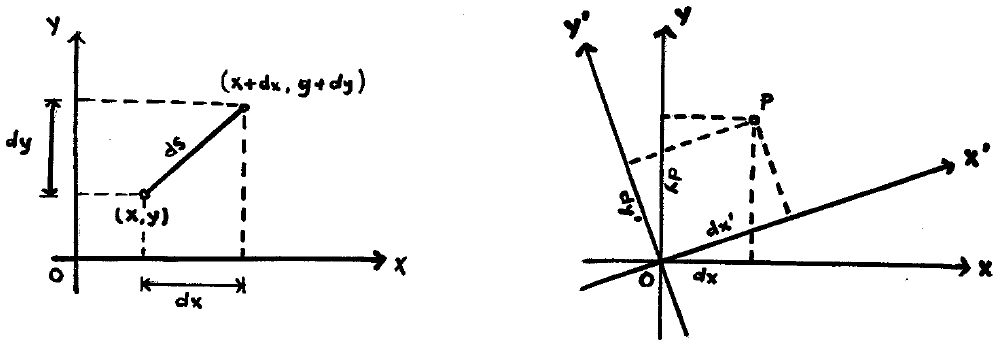
\includegraphics[scale=0.6]{Draw/lec2_6.png}
\end{center}
\caption{Euclidean space}
\label{fig:lec2_6}
\end{figure}

Next we introduce some useful notation. We write the coordinates $x$, $y$, $z$ as $x^i$, where the index $i=1,2,3$. In other words, we define
\begin{equation}
\begin{split}
x^1&\equiv x,\\
x^2&\equiv y,\\
x^3&\equiv z.
\end{split}
\end{equation}
Remember, the $i$ on $x^i$ is simply an index, not a power. The reason for writing it as an upper index will become clear later. We will also denote as $\delta_{ij}$ the components of the $3\times3$ identity matrix:
\begin{equation}
I=\left( \begin{array}{ccc} 1 & 0 & 0 \\ 
0 & 1 & 0 \\
0 & 0 & 1 \end{array} \right)
\end{equation}
The index $i$ on $\delta_{ij}$ denotes de row, and the index $j$ denotes de column. For example, $\delta_{21}$ represents the entry on the 2nd row and 1st column of $I$, which we see is zero. Clearly we have
\begin{equation}
\delta_{ij}=\begin{cases} 1, & \mbox{if $i=j$} \\ 
0, & \mbox{if $i\neq j$} \end{cases}
\end{equation}
Let us now multiply $\delta_{ij}$ with $dx^i dx^j$ and sum over all values of $i$ and $j$:
\begin{equation}
\begin{split}
\sum_{i=1}^3\sum_{j=1}^3 \delta_{ij}dx^i dx^j &= \delta_{11}(dx^1)^2+\delta_{22}(dx^2)^2+\delta_{33}(dx^3)^2\\
&= dx^2+dy^2+dz^2,
\end{split}
\end{equation}
which is precisely the right hand side of eq.\ (\ref{eq:euclid_line_elem}). We will simplify the notation by introducing now the {\it Einstein summation convention} (see also Chapter 1): whenever an expression contains one index as a superscript and the {\it same} index as a subscript, a summation is implied over all values the index can take. With this convention we can then write
\begin{equation} \label{eq:euclidean_metric}
ds^2=\delta_{ij}dx^i dx^j.
\end{equation}
The space where distances are measured using eq.\ (\ref{eq:euclidean_metric}) is called Euclidean space. The tensor $\delta_{ij}$ is called the {\it metric} of Euclidean space.

\par\vspace{\baselineskip}

{\bf Exercise.} Here is an exercise so that you start getting used to the Einstein summation convention. Let $M_{ij}$ be the components of the matrix
\begin{equation}
M=\left( \begin{array}{ccc} 1 & 2 & -1 \\ 
3 & 0 & -2 \\
2 & 4 & 1 \end{array} \right),
\end{equation}
let $a^i$ be the components of the vector $\mathbf{a}=(2,-1,0)$, and let $b^i$ be the components of the vector $\mathbf{b}=(-1,0,-2)$. Show that $M_{ij}a^ib^j=1$.

\par\vspace{\baselineskip}

An obvious but important property of $ds^2$ is that it is invariant under coordinate transformations. This is very intuitive: the distance between two points in space cannot depend on how we set up the $x$, $y$ and $z$ axes. We could even choose a different set of coordinates, for instance spherical coordinates, and the distance should obviously not change. In the example of fig.\ \ref{fig:lec2_6} we have rotated the $x$ and $y$ axes into the $x'$ and $y'$ axes (we are in 2 dimensions now). The distance $ds$ from the origin $O$ to the point $P$ has components $dx$ and $dy$ along the $x$ and $y$ axes, and components $dx'$ and $dy'$ along the $x'$ and $y'$ axes. Note that $dx\neq dx'$ and $dy\neq dy'$, but $dx^2+dy^2=dx'^2+dy'^2$, meaning that $ds^2$ is the same in both coordinate systems.

\subsection{Minkowski spacetime}

How do we measure ``distances'' in spacetime? We would like to define some sort of distance between two events (i.e.\ two points in spacetime) that is independent of the reference frame, just like the Euclidean distance is independent of the orientation of axes. We already know the answer: we have seen above that the spacetime interval $\Delta s^2$ between two events remains invariant when going from one inertial frame to another. Taking $\Delta s$ to be infinitesimal we can write down the spacetime interval in terms of differentials as
\begin{equation}
ds^2=-c^2dt^2+dx^2+dy^2+dz^2.
\end{equation}
Next we simplify the notation as we did in the case of 3 dimensions. We use the same notation for the spatial coordinates, and introduce the coordinate $x^0=ct$. In summary, the 4 coordinates we will use to describe spacetimes will be then
\begin{equation}
\begin{split}
x^0&\equiv ct,\\
x^1&\equiv x,\\
x^2&\equiv y,\\
x^3&\equiv z.
\end{split}
\end{equation}
Define the matrix
\begin{equation}
\label{etamunu}
\eta=\left( \begin{array}{cccc} -1 & 0 & 0 & 0 \\ 
0 & 1 & 0 & 0 \\
0 & 0 & 1 & 0 \\
0 & 0 & 0 & 1\end{array} \right).
\end{equation}
The components of this matrix are denoted by $\eta_{\mu\nu}$, where the indices $\mu$ and $\nu$ range from $0$ to $3$. (The convention is that latin indices are restricted to the spatial coordinates, so they range from 1 to 3, whereas greek indices are used for spacetime coordinates, so they also include the time or zeroth component.) If we multiply $\eta_{\mu\nu}$ by $dx^{\mu}dx^{\nu}$ and sum over all values of $\mu$ and $\nu$, we get
\begin{equation}
\begin{split}
\eta_{\mu\nu}dx^{\mu}dx^{\nu}&\equiv \sum_{\mu=0}^3\sum_{\nu=0}^3 \eta_{\mu\nu}dx^{\mu}dx^{\nu}\\
&=\eta_{00}(dx^0)^2+\eta_{11}(dx^1)^2+\eta_{22}(dx^2)^2+\eta_{33}(dx^3)^2\\
&=-c^2dt^2+dx^2+dy^2+dz^2,
\end{split}
\end{equation}
which is precisely equal to the spacetime interval. We conclude that
\begin{equation} \label{eq:mink_metric}
ds^2=\eta_{\mu\nu}dx^{\mu}dx^{\nu}.
\end{equation}
The spacetime where intervals between events are measured using eq.\ (\ref{eq:mink_metric}) is called Minkowski spacetime. The tensor $\eta_{\mu\nu}$ is called the metric of Minkowski spacetime.

Just as the squared distance $ds^2$ of Euclidean space is invariant under rotations of the coordinate axes, so the interval $ds^2$ of Minkowski spacetime is invariant under Lorentz transformations. Actually, the invariance of $ds^2$ is a stronger statement. In Euclidean space $ds^2$ is not only invariant under rotations of axes, but also under a general coordinate transformation. The difference is that, whereas in the case of a rotation of axes the metric $\delta_{ij}$ does not change,\footnote{We saw in the example of fig.\ \ref{fig:lec2_6} that $ds^2=dx^2+dy^2=dx'^2+dy'^2$, which can be written as $ds^2=\delta_{ij}dx^idx^j=\delta_{ij}dx'^idx'^j$ (with $dz=dz'=0$ in 2 dimensions). In other words, the metric is the same in the two coordinate systems, namely $\delta_{ij}$.} in the general case the metric will change when going from one coordinate system to another. Similarly, in Minkowski spacetime the metric $\eta_{\mu\nu}$ does not change when going from one inertial frame to another, since inertial frames 
are always connected by Lorentz transformations, but it will change if we go to more general reference frames, such as accelerated frames. As we will see in the next lecture, Einstein noted the equivalence between an accelerated frame and a frame subject to a gravitational field. This observation led him to establish a deep connection between the metric of spacetime and the gravitational field, which is the basis of General Relativity.
